\newcommand{\radius}{1 cm}
\newcommand{\qpt}{8 $\mu$C}
\newcommand{\Q}{5 $\mu$C}
\newcommand{\qloc}{$<1.5,0,0>$ cm}
\newcommand{\rone}{$<0,0.5,0>$ cm}
\newcommand{\rtwo}{$<0,5,0>$ cm}
\question An insulating sphere of radius $R$ = \radius{} lies with its center at the origin. The sphere has positive charge of $Q$ = \Q{} spread uniformly over its surface. A point charge with charge \qpt{} lies on the $x-$axis at \qloc. You may neglect the polarization of the insulator (assume the polarizability$\alpha$ is 0)

\begin{center}
	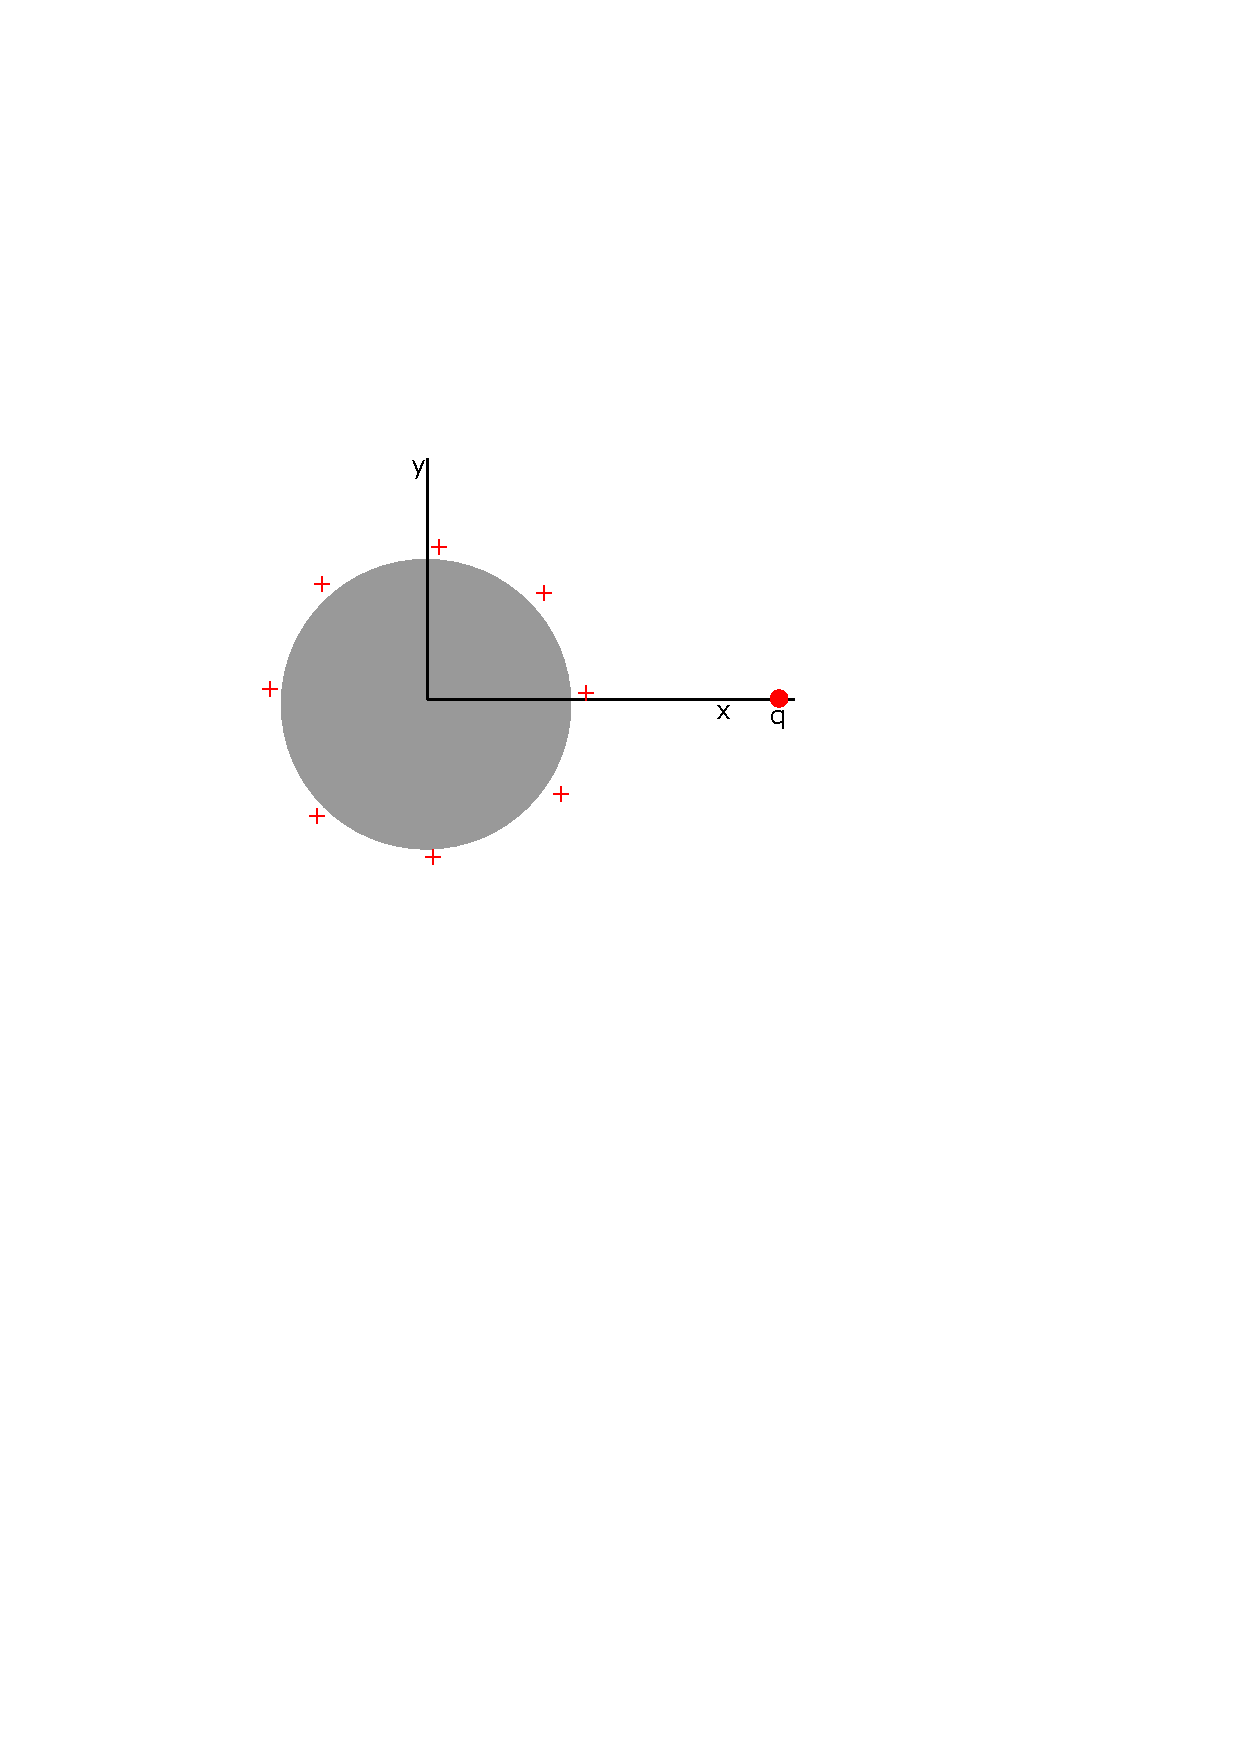
\includegraphics[width=6cm]{charge_and_sphere.pdf}
\end{center}

\begin{parts}
	\part What is the net electric field at the point \rone{} (inside the sphere)?
	\vspace{3cm}
	\part What is the net electric field at the point \rtwo{} (outside the sphere)?
	\vspace{3cm}
	\part The insulating sphere is now replaced with a conducting sphere with the same charge ($Q$ = \Q{}). What is the net electric field at the point \rone?
	\vspace{3cm}
	\part What is the induced electric field due to the polarized conductor at \rone?
\end{parts}